\documentclass[a4paper,12pt]{article} 
\usepackage{geometry}
\geometry{
	a4paper,
	total={170mm,257mm},
	left=20mm,
	top=20mm,
}
\usepackage{titlesec}
\titlelabel{\thetitle.\quad} %точка в section

%%% Работа с русским языком
\usepackage{cmap}                           % поиск в PDF
\usepackage{mathtext} 			 	       % русские буквы в формулах
\usepackage[T2A]{fontenc}               % кодировка
\usepackage[utf8]{inputenc}              % кодировка исходного текста
\usepackage[english,russian]{babel}  % локализация и переносы

%Математика
\usepackage{amsmath,amsfonts,amssymb,amsthm,mathtools} % AMS
\usepackage{icomma} % "Умная" запятая

%% Шрифты
\usepackage{euscript}	 % Шрифт Евклид
\usepackage{mathrsfs} % Красивый матшрифт

%% Команды
\DeclareMathOperator{\const}{\mathop{const}}

%% Перенос знаков в формулах
\newcommand*{\hm}[1]{#1\nobreak\discretionary{}
	{\hbox{$\mathsurround=0pt #1$}}{}}

%%% Заголовок
\author{Шерхалов Денис Б02-204}
\title{Лабораторная работа 2.2.6 \\
	\textbf{Определение энергии активации по температурной зависимости вязкости жидкости}}
\date{\today}

\begin{document}
	
	{\Large \maketitle}

	\paragraph*{Цель работы:} 1) измерение скорости падения шариков при разной температуре жидкости; 2) вычисление вязкости жидкости по закону Стокса и расчет энергии активации.
	
	\paragraph*{В работе используются:} стеклянный цилиндр с исследуемой жидкостью (глицерин); термостат; секундомер; горизонтальный компаратор; микроскоп; мелкие шарики (диаметром 1-2 мм).
	
	\section{Введение}
	Для того чтобы перейти в новое состояние, молекула жидкости должна преодолеть участки с большой потенциальной энергией, превышающей среднюю тепловую энергию молекул. Для этого тепловая энергия молекул должна — вследствие флуктуации — увеличиться на некоторую величину $W$ , называемую энергией активации. Температурная зависимость вязкости жидкости при достаточно грубых предположениях можно описать формулой
	\begin{equation} \label{activation_energy:1}
		\eta \sim A e^{W/kT}
	\end{equation}
	
	Из формулы (\ref{activation_energy:1}) следует, что существует линейная зависимость между величинами $\ln\eta$ и $1/T$, и энергию активации можно найти по формуле
	
	\begin{equation} \label{activation_energy:2}
		W = k \frac{d(\ln\, \eta)}{d(1/T)}
	\end{equation}
	
	По формуле Стокса, если шарик радиусом $r$ и со скоростью $v$ движется в среде с вязкостью $\eta$, и при этом не наблюдается турбулентных явлении, тормозящую силу можно найти по формуле (\ref{stokes})
	
	\begin{equation}\label{stokes}
		F = 6\pi\eta rv
	\end{equation}
	
	Для измерения вязкости жидкости рассмотрим свободное падение шарика в жидкости. При медленных скоростях на шарик действуют силы Архимеда и Стокса, выражения для которых мы знаем. Отсюда находим выражения для установившейся скорости шарика и вязкости жидкости
	
	\begin{align}
		v_{уст}&=\frac{2}{9}gr^2\frac{\rho - \rho_ж}{\eta}\label{v_ust},\qquad \tau = \frac{2r^2\rho}{9\eta}
	\end{align}

	\begin{align}
		\eta&=\frac{2}{9}gr^2\frac{\rho - \rho_ж}{v_{уст}}\label{eta}
	\end{align}

	\begin{equation*}
		Re = \dfrac{\rho_{ж} v d}{\eta}, \qquad S = v_{уст} \tau
	\end{equation*}

	Как видим, измерив установившуюся скорость шарика и параметры системы можно получить вязкость по формуле (\ref{eta}).
	
	
	\subparagraph*{Экспериментальная установка}
	Для измерений используется стеклянный цилиндрчиеский сосуд B, наполненный исследуемой жидкостью (глицерин). Диаметр сосуда $\approx 3$ см, длина $h = 20$ см. На стенках сосуда нанесены две метки на некотором расстоянии друг от друга. Верхняя метка должна располагаться ниже уровня жидкости с таким расчетом, чтобы скорость шарика к моменту прохождения этой метки успевала установиться. Измеряя расстояние между метками, b время падения определяют установившуюся скорость шарика $v_{уст}$. Сам сосуд B помещен в рубашку D, омываемую водой из термостата. При работающем термостате температура воды в рубашке D, а потому и температура жидкости 12 равна температуре воды в термостате.
	Схема прибора (в разрезе) показана на рис.1.
	
	\begin{figure}[h!]
		\centering{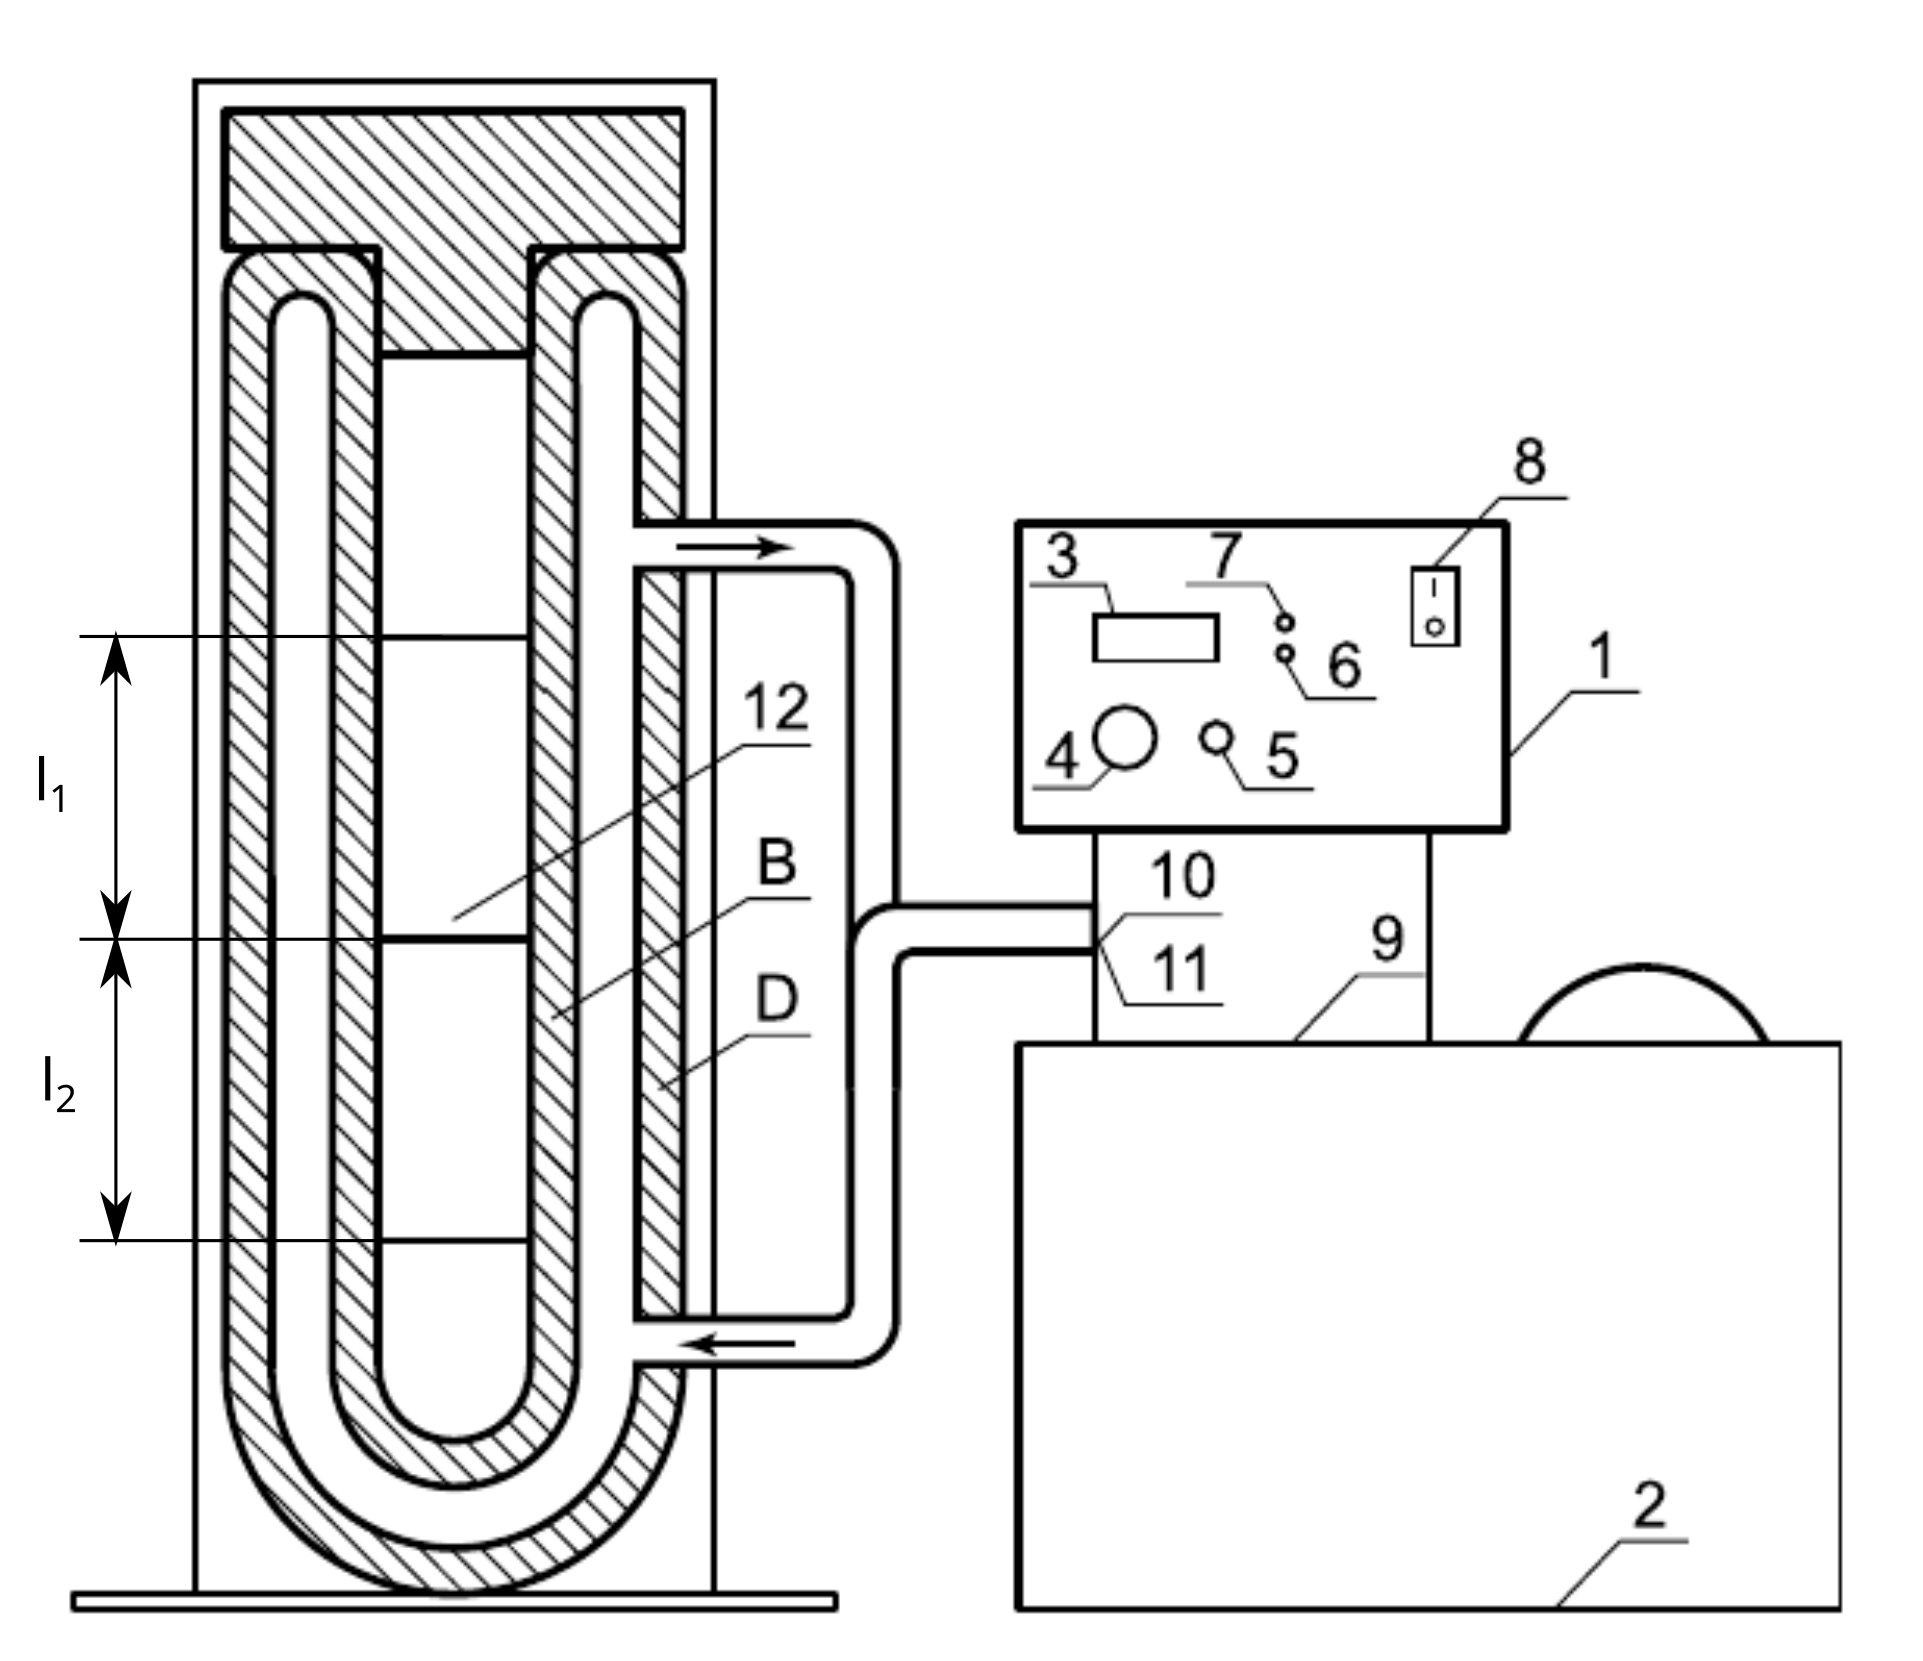
\includegraphics[width=0.5\textwidth]{pic1.png}}
		\caption[]{\label{fig:1} Установка для определения коэффициента вязкости жидкости.}
	\end{figure}

	\begin{figure}[h!]
		\centering{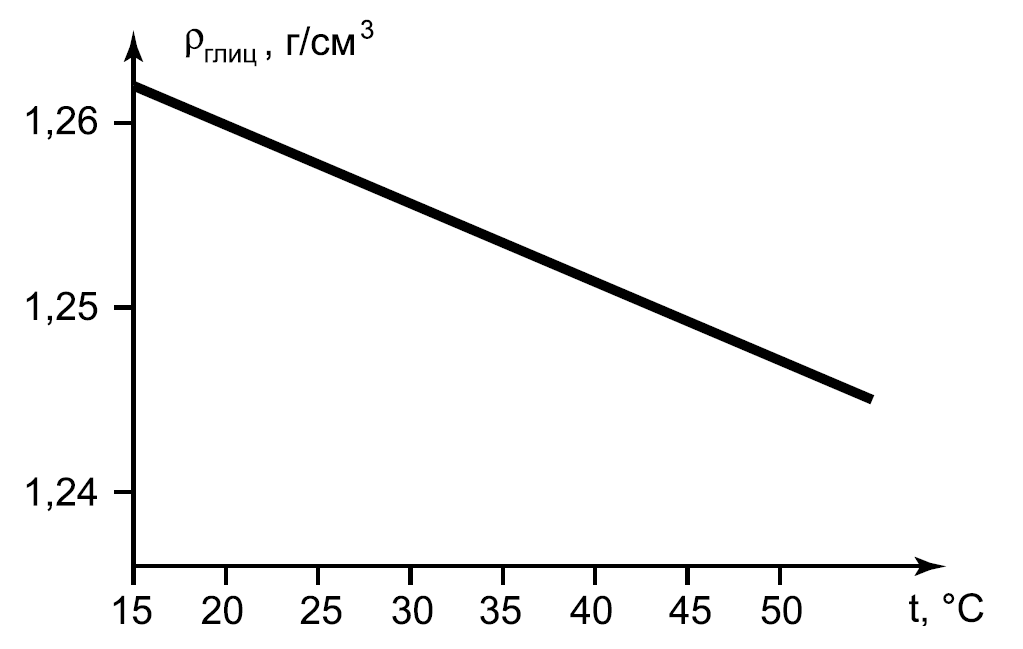
\includegraphics[width=0.5\textwidth]{pic2.png}}
		\caption[]{\label{fig:2} Зависимость плотности  глицерина от температуры.}
	\end{figure}
	
	\newpage
	
	\section{Выполнение}
	\begin{enumerate}
		\item Отберём 20 шариков -- 10 стеклянных и 10 стальных. Измерим их размеры с помощью микроскопа. Будем измерять в двух перпендикулярных плоскостях и усреднять. 
		$$\rho_{стекло} = 2.5 \, ^{г}/_{см^3} \qquad \rho_{сталь} = 7.8 \, ^{г}/_{см^3}$$
	
		\item Измерим установившиеся скорости падения шариков и вычислим вязкость $\eta$ по  формуле (5). Измерения выполним для 5 значений температуры в  интервале  от  комнатной до $60^\circ C$. Для каждого значения температуры определим плотность жидкости $\rho_{ж}$ по графику, приложенному к работе (рис. 2).
		\begin{table}[h!] 
			\caption{Значение плотности глицерина в зависимости от температуры}
			\begin{center}
				\begin{tabular}{|*{6}{l|}} \hline
					$Т$, $^\circ C$ & 20.5 & 31.0 & 40.8 & 50.1 & 60.0 \\ \hline
					$\rho_{ж}$, $^г/_{см^3}$ & 1.260 & 1.255 & 1.250 & 1.245 & 1.240 \\ \hline
				\end{tabular}
			\end{center}
		\end{table}
	
		\item Оценим погрешности:
		$$\Delta t_{пад} = 0.2\,c, \qquad \Delta T = 0.5\,K$$
		$$\Delta v_{уст} = \Delta t_{пад} \, \dfrac{h}{t^2_{пад}}$$
		$$\Delta\eta =\dfrac{2}{9}gr^2 \, \dfrac{\rho - \rho_ж}{v^2_{уст}} \Delta v_{уст} $$
	
		\begin{table}
		\caption{Измерения времени для стальных шариков}
		\begin{center}
			\begin{tabular}{|l|l|l|l|rr|rr|lll|}
				\hline
				{№} & {$T, ^\circ C$} & {$d, мм$} & {$t_{пад}, с$} & {$v, см/с$} & {$\Delta v, см/с$} & {$\eta, мПа \cdot с$} & {$\Delta\eta, мПа \cdot с$} &  {$\tau, мс$} & {Re} & {$S, \mu м$} \\
				\hline
				1 & 20.5 & 0.80 & 81.77 & 0.245 & 0.001 & 933 & 2 & 0.30 & 0.003 & 0.73 \\
				2 &      & 0.90 & 72.55 & 0.276 & 0.001 &1048 & 3 & 0.33 & 0.003 & 0.92 \\ \hline
				3 & 31.0 & 0.70 & 69.66 & 0.287 & 0.001 & 609 & 2 & 0.35 & 0.004 & 1.00 \\
				4 &      & 0.70 & 63.06 & 0.317 & 0.001 & 551 & 2 & 0.39 & 0.005 & 1.22 \\ \hline
				5 & 40.8 & 0.80 & 29.34 & 0.682 & 0.004 & 335 & 2 & 0.83 & 0.020 & 5.64 \\
				6 &      & 0.90 & 23.41 & 0.854 & 0.007 & 339 & 3 & 1.04 & 0.028 & 8.86 \\ \hline
				7 & 50.1 & 0.85 &  9.82 & 2.037 & 0.041 & 127 & 3 & 2.47 & 0.170 & 50.3 \\
				8 &      & 0.88 & 10.02 & 1.996 & 0.040 & 139 & 3 & 2.42 & 0.158 & 48.3 \\ \hline
				9 & 60.0 & 0.80 &  6.03 & 3.317 & 0.110 &  69 & 2 & 4.02 & 0.477 & 133.3 \\
				10 &     & 0.65 &  9.60 & 2.083 & 0.043 &  73 & 2 & 2.52 & 0.231 & 52.6 \\ \hline
			\end{tabular}
		\end{center}
	\end{table}

	\begin{table}
		\caption{Измерения для стеклянных шариков}
		\begin{center}
			\begin{tabular}{|l|l|l|l|rr|rr|lll|}
				\hline
				{№} & {$T, ^\circ C$} & {$d, мм$} & {$t_{пад}, с$} & {$v, см/с$} & {$\Delta v, см/с$} & {$\eta, мПа \cdot с$} & {$\Delta\eta, мПа \cdot с$} &  {$\tau, мс$} & {Re} & {$S, \mu м$} \\
				\hline
				1 & 20.5 & 2.00 & 67.28 & 0.297 & 0.001 & 910 & 3 & 0.611 & 0.008 & 1.82 \\
				2 &      & 2.05 & 68.60 & 0.292 & 0.001 & 975 & 3 & 0.599 & 0.008 & 1.75 \\ \hline
				3 & 31.0 & 2.00 & 36.16 & 0.553 & 0.003 & 491 & 3 & 1.132 & 0.028 & 6.26 \\
				4 &      & 2.10 & 36.03 & 0.555 & 0.003 & 539 & 3 & 1.136 & 0.027 & 6.30 \\ \hline
				5 & 40.8 & 2.05 & 18.39 & 1.088 & 0.012 & 263 & 3 & 2.216 & 0.106 & 24.10 \\
				6 &      & 2.10 & 17.88 & 1.119 & 0.013 & 269 & 3 & 2.279 & 0.109 & 25.49 \\ \hline
				7 & 50.1 & 2.05 &  8.70 & 2.299 & 0.053 & 125 & 3 & 4.665 & 0.469 & 107.3 \\
				8 &      & 2.05 &  8.80 & 2.273 & 0.052 & 127 & 3 & 4.612 & 0.458 & 104.8 \\ \hline
				9 & 60.0 & 2.05 &  5.44 & 3.676 & 0.135 &  79 & 3 & 7.432 & 1.190 & 273.2 \\
				10 &     & 2.10 &  5.29 & 3.781 & 0.143 &  80 & 3 & 7.642 & 1.228 & 288.9 \\ \hline
			\end{tabular}
			\end{center}
	\end{table}

	\item Теперь построим график $\ln \, \eta (T^{-1})$ (График №1).
	\begin{figure}[h!]
		\centering{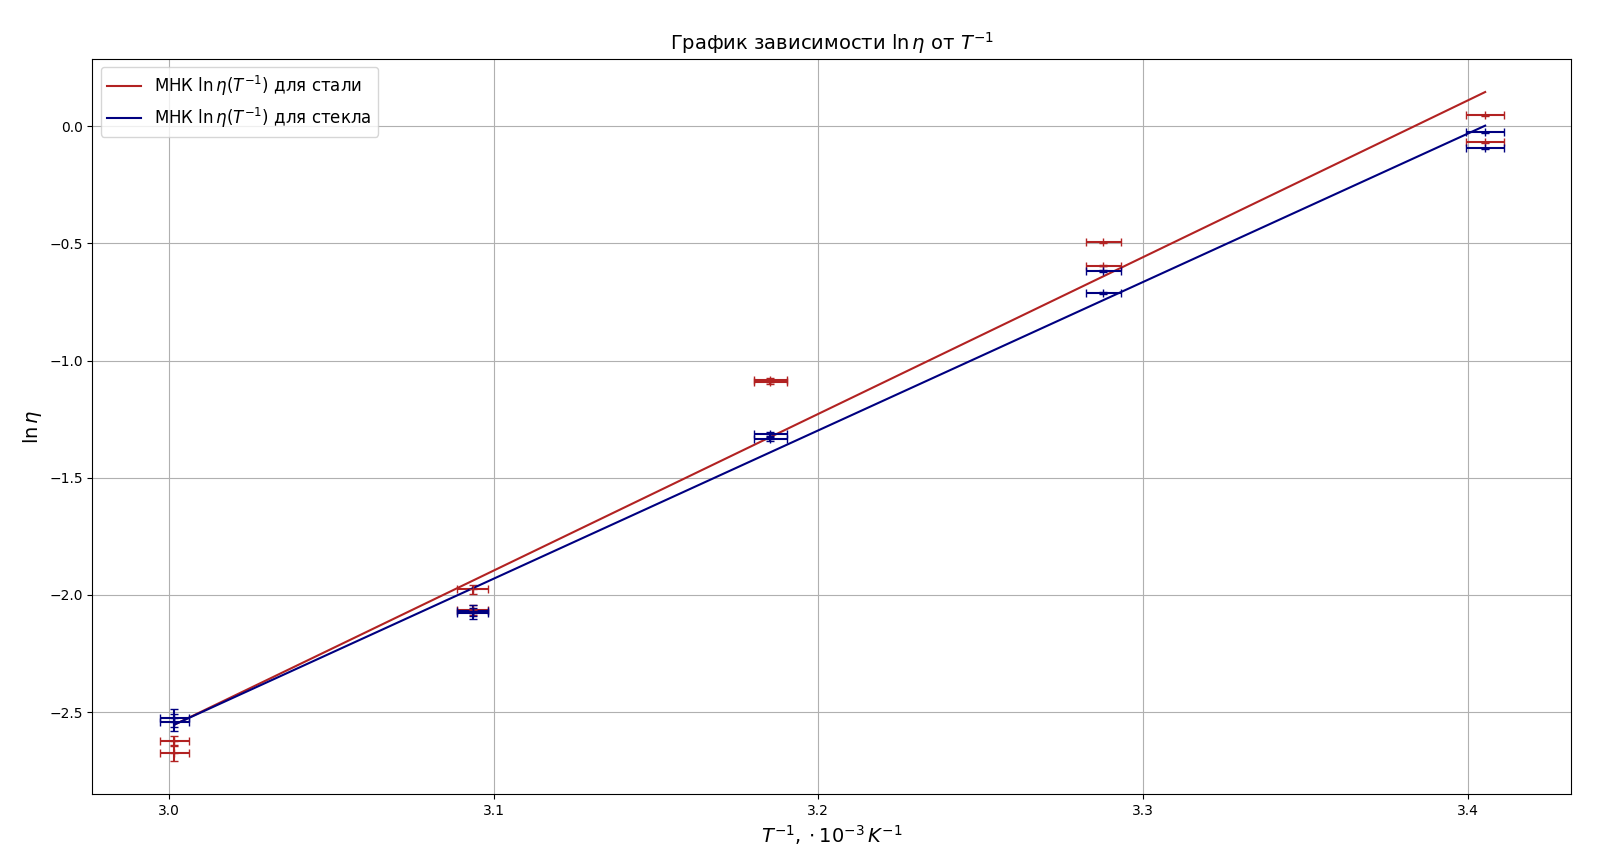
\includegraphics[width=1.00\textwidth]{gr1.png}}
		\caption[]{\label{fig:3} График №1 $\ln \, \eta (T^{-1})$}
	\end{figure}
	$$\left(\dfrac{d(\ln\, \eta)}{d(1/T)}\right)_{сталь} = (6686 \pm 142)\, K \; \Rightarrow \; W_{сталь}/k = (6686 \pm 142)\, K$$
	$$\left(\dfrac{d(\ln\, \eta)}{d(1/T)}\right)_{стекло} = (6329 \pm 36),\, K \; \Rightarrow \; W_{стекло}/k = (6361 \pm 36)\, K$$
	$$\left(\dfrac{d(\ln\, \eta)}{d(1/T)}\right)_{средн} = (6524 \pm 162),\, K \; \Rightarrow \; W_{средн}/k = (6524 \pm 162)\, K$$

\end{enumerate}

\newpage 

\section{Вывод}
	Во-первых, так как в каждом опыте значение числа Рейнольдса $Re$ было очень маленьким (меньше $1.5$), поэтому можно считать, что обтекание шарика жидкостью действительно имело ламинарный характер и формула Стокса справедлива в данной лабораторной работе. 

	Так же мы вычислили вязкость исследуемой жидкости (глицерина) по закону Стокса, например при $T = 323$ К $\eta = (130\, \pm \, 7)$ мПа$\cdot$с, что соотвествует табличному значению раствора глицерина.
	И вычислили энергию активации глицерина $W =(90 \pm 2)$ зептоДж.

\end{document}